The electronics that modern computers rely on contain components that operate based on quantum mechanics; however, their computational processes are still governed by classical laws. 
For this reason, they are referred to as "classical computers."\\

Quantum computing emerged from Richard Feynman’s idea that simulating quantum systems efficiently requires quantum mechanical resources \cite{Feynman1982}. 
Classical computers struggle to model complex quantum interactions due to the exponential growth of computational requirements with system size, making exact simulations infeasible beyond small systems \cite{Brown2010}. 
Quantum computers, taking advantage of quantum mechanics phenomena like superposition and entanglement, offer a natural framework for such simulations and have been demonstrated to provide exponential speedups for certain quantum systems \cite{Georgescu_2014}.

Beyond quantum simulation, curren theoretical advancements suggest that quantum algorithms can outperform classical counterparts in solving specific problems \cite{Montanaro2016}.

\section{Introduction}
The physical realization of quantum computing necessitates the development of a system capable of functioning as quantum bits (qubits).\\
Similar to classical logic, where the bits 0 and 1 are associated with two physical levels, typically represented by high and low voltage states, a qubit can, to a first approximation, be considered as a two-level physical system.

Mathematically, this system is described within a two-dimensional complex Hilbert space, where the basis states $\ket{0}$ and $\ket{1}$ correspond to two orthonormal vectors.
Any general state of the qubit can be expressed as a superporition of these basis states:
\begin{equation}\label{eq:qubit}
    \ket{\psi} = \alpha\ket{0} + \beta\ket{1} \rightarrow \begin{pmatrix} 
        \alpha \\ 
        \beta 
        \end{pmatrix},
\end{equation}
where $\alpha,\beta\in \mathbb{C}$. If the normalization condition $|\alpha|^2 +|\beta|^2 =1$ holds, the state $\ket{\psi}$ represents a qubit.
The basis $\{\ket{0},\ket{1}\}$ is called computational basis and the information is stored in the complex numbers $\alpha$ and $\beta$.

\paragraph{}
A possible geometric representation of qubit states is given by the Bloch sphere, which offers a visualization of two level quantum systems as vectors on a unit sphere.  
A qubit state is depicted as a vector originating from the center of the sphere, with the computational basis states $\ket{0}$ and $\ket{1}$ positioned at the north and south poles, respectively.
The axis connecting these states defines the $z$-axis. The transverse $x$- and $y$- axes correspond to the equal superposition states $\ket{\pm} = \frac{1}{\sqrt{2}}(\ket{0}\pm\ket{1})$ and $\ket{\pm i} = \frac{1}{\sqrt{2}}(\ket{0}\pm i\ket{1})$, respectively.\\
A vector of unit length on the Blooch sphere is characterized by the polar angle $\theta$, with $0\leq\theta\leq\pi$ and the azimuthal angle $\varphi$, with $0\leq\varphi\leq 2\pi$, each unit vector represent a possible pure state of the qubit.\\

\begin{figure}[h!]
\centering
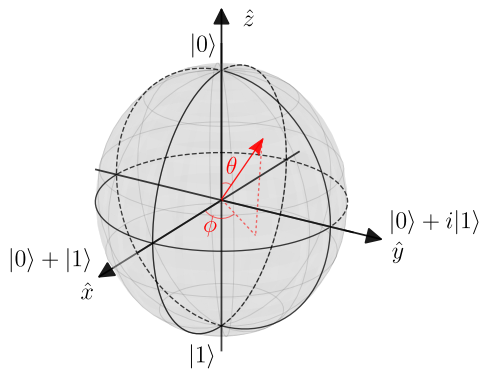
\includegraphics[width=0.25\textwidth]{figures/png/BlochSphere.png}
\caption{Example of qubit state representation on the Bloch sphere\\
Source: Metrology of Quantum Control and Measurement in Superconducting Qubits \cite{Chen2018}}
\label{fig:BlochSphere}
\end{figure}

The qubit states $\ket{0}$ and $\ket{1}$ can also be associated with energy eigenstates of a physical system, where $\ket{0}$ represents the ground state with energy $E_0$ and $\ket{1}$ represents the excited state with energy $E_1$, assuming $E_0 < E_1$. 
In this energy eigenbasis, the Hamiltonian of the qubit is given by
\begin{equation}\label{eq:qubithamiltonian}
    \hat{H}_q = E_0 \ket{0} \bra{0} + E_1 \ket{1} \bra{1} = 
    \begin{pmatrix}
        E_0 & 0 \\
        0 & E_1
    \end{pmatrix}.
\end{equation}

Since only energy differences are physically relevant, it is possible to redefine the zero-point energy by subtracting the constant term $E_0 (\ket{0} \bra{0} + \ket{1} \bra{1})$, leading to the simplified Hamiltonian
\begin{equation}\label{eq:qubithamiltonian}
    \hat{H}_q = (E_1 - E_0) \ket{1} \bra{1} = \hbar \omega_q \ket{1} \bra{1} = \hbar \omega_q \hat{\sigma}^{+} \hat{\sigma}^{-} = 
    \begin{pmatrix}
        0 & 0 \\
        0 & \hbar \omega_q
    \end{pmatrix},
\end{equation}

where $\omega_q = (E_1 - E_0)/\hbar$ is the qubit transition frequency, and we have used the relation $\hat{\sigma}^{+} \hat{\sigma}^{-} = \ket{1} \bra{1}$.
For convenience, the Hamiltonian can also be rewritten in terms of the Pauli $z$-matrix, $\hat{\sigma}_z$, by adding a term proportional to the identity:
\begin{equation}
    \hat{H}_q = \hbar \omega_q \ket{1} \bra{1} - \frac{\hbar \omega_q}{2}\mathbb{I} = 
    \begin{pmatrix}
        -\frac{\hbar \omega_q}{2} & 0 \\
        0 & \frac{\hbar \omega_q}{2}
    \end{pmatrix} = -\frac{\hbar \omega_q}{2} \hat{\sigma}_z.
\end{equation}

\paragraph{}
Qubits can be implemented through various physical mechanisms; however, their practical realization remains a significant challenge due to their susceptibility to environmental interactions, which lead to decoherence and reduce their coherence time. 
Despite the diversity of possible physical implementations, any functional quantum computing system must satisfy a set of fundamental criteria. 
These requirements, known as the DiVincenzo criteria, establish the essential conditions for the construction and operation of a viable quantum computer \cite{DiVincenzo_2000}, \cite{manenti_quantum_2023}:
\begin{enumerate}
    \item The physical system used as quantum computer must comprise a set of qubits, meaning that the quantum system must be well-characterized, and scalable such that quantum
    computing can be realized.
    \item It must be possible to initialize the qubits in a reliable state, such as the ground state.
    \item The coherence time of the qubits must be longer than the typical gate time.
    \item It must be possible to implement a universal set of quantum gates.
    \item It must be possible to measure the qubits in the computational basis.
\end{enumerate}

In the present work, I will focus on superconducting qubits, which constitute the hardware I have worked on and where the experiments were conducted. 
However, several of the experiments described later can also be implemented using different physical systems.

\section{Transmon qubits}\label{sec:cQED}
In questa sezione faccio un ripasso della struttura e del funzionamento dei superconducting transmon qubits, per la stesura di questa sezione ho fatto riferimento al Qunatum Information Science manual \cite{manenti_quantum_2023}, the Metrology of Quantum Control and Measurement in Superconducting Qubits \cite{Chen2018} and the original paper \cite{TransmonPaper}.

A transmon consists of two superconducting pads connected by a Josephson junction. 
The Josephson junction (JJ) is formed by a thin oxide layer positioned between the two superconductors which acts as an insulating barriers. 

Superconductivity is a phenomenon observed in certain materials where, when cooled well below a critical temperature $T_c$, which depends on the material, their electrical resistance drops to zero, allowing them to behave as perfect conductors.
According to the BCS (Bardeen-Cooper-Schrieffer) theory, superconductivity arises, from the formation of Cooper pairs, which are bound states of electrons with opposite momenta and spins.
These pairs collectively forms a macroscopic quantum states described by a single waveform $\psi(\mathbf{r})$ which can be expressed as 
\begin{equation}\label{eq:BCSequation}
    \psi(\mathbf{r}) = \sqrt{\rho(\mathbf{r})}e^{i\theta(\mathbf{r})}
\end{equation}
where $\rho(\mathbf{r})$ is the density of Cooper pairs in the metal, which is typically uniform in the bulk of the superconductor, and $\theta(\mathbf{r})$ is the macroscopic phase of the superconducting wavfunction.

For this reason the wavefunctions on the two sides of the JJ can be denoted as
\begin{equation}\label{eq:JosephsonWavefunctions}
    \psi_1(\mathbf{r}, t) = \sqrt{\rho_1(\mathbf{r}, t)} e^{i\theta_1(\mathbf{r},t)}, \psi_2(\mathbf{r}, t) = \sqrt{\rho_2(\mathbf{r}, t)} e^{i\theta_2(\mathbf{r},t)}
\end{equation}

The dynamics of the system can be described by the two equations\begin{equation}\label{eq:schr1}
    i\hbar \frac{d\psi_1}{dt} = E_1 \psi_1 + K \psi_2,
\end{equation}
\begin{equation}\label{eq:schr2}
    i\hbar \frac{d\psi_2}{dt} = E_2 \psi_2 + K \psi_1.
\end{equation}
By substituting the expression of $\psi_i$ into the Schr\"odinger equation \ref{eq:schr1}, \ref{eq:schr2} we obtain
\begin{equation}\label{eq:schr-sub1}
    \frac{d\rho_1}{dt} = \frac{2K}{\hbar} \sqrt{\rho_1 \rho_2} \sin(\theta_2 - \theta_1),
\end{equation}
\begin{equation}\label{eq:schr-sub2}
    \frac{d\rho_2}{dt} = -\frac{2K}{\hbar} \sqrt{\rho_1 \rho_2} \sin(\theta_2 - \theta_1).
\end{equation}

Since the derivative of the charge density is the current, from equations \ref{eq:schr-sub1} and \ref{eq:schr-sub2} we obtain the first Josephson equation
\begin{equation}\label{eq:Josephson1}
    I=I_c\sin{\phi}
\end{equation} 
where $I_c = \frac{2K}{\hbar}\sqrt{\rho_1\rho_2}$ is the critical current and $\phi$ is the superconducting phase difference $\theta_2 - \theta_1$.

Instead, from the real part of the Schr\"odinger equation \ref{eq:schr1}, \ref{eq:schr2} and a few calculations, we obtain the second Josephson equation
\begin{equation}\label{eq:Josephson2}
    \frac{d\phi}{dt} = \frac{2e}{\hbar} V(t).
\end{equation}
which can be rewritten as \begin{equation}
    \frac{d\phi}{dt} = \frac{2\pi}{\Phi_0} V(t).
\end{equation}
where $\Phi_0$ is the superconducting flux quantum.
The frequency $f_Q$ of a two-junction transmon dependends on the magnetic flux $\Phi_Q(t)$ through the SQUID loop, for symmetric junctions is given by\cite{TransmonPaper}
\begin{equation}\label{eq:freqdepndenceonflux}
    f_Q(\Phi_Q) \approx \frac{1}{h} \left( \sqrt{8E_J E_C \cos\left(\pi \frac{\Phi_Q}{\Phi_0} \right)} - E_C \right)    
\end{equation}

where $E_C$ is the charging energy, $E_J$ is the sum of the Josephson energies of the individual Josephson junctions, $\Phi_0$ is the flux quantum, and $h$ is the Planck's constant.

\subsection{Density matrix}
%Posso rappresentatre l'operatore densità come una matrce 2x2, mi serve per dopo, per la descrizione del depolarizing channel
\section{Quantum operations}
A quantum operation is a mathematical transformation that describes how a quantum state changes as a consequence of a physical process. Formally, it is a map $\mathcal{E}$ that transforms a quantum state described by a density operator $\hat{\rho}$ into another state described by a new density operator $\hat{\rho}'$:
\begin{equation}
    \mathcal{E}(\rho) = \rho'\label{eq:quantum_map}.
\end{equation}

The simplest example of a quantum operation is the evolution of a quantum state $\hat{\rho}$ of a closed quantum system, under a unitary operator $\hat{U}$, which can be written as $\mathcal{E} \equiv \hat{U} \hat{\rho} \hat{U}^{\dagger}$.

\paragraph{Depolarizing chennel}
A depolarizing channel describes a process in which the current state of the $n$-qubit system $\rho$, is replaced by $\frac{\id}{2^n}$, with probability $d$. This process can be represented with a quantum map as follows:
\begin{equation}
    \mathcal{E}_{dc}(\rho) = d\frac{\id}{2^n}+(1-d)\rho\label{eq:depolarizing_channel}
\end{equation} 


\subsection{Rabi experiments}


